%%%%%%%%%%%%%%%%%%%%%%%%%%%%%%

%%% SAMPLE_IJAM file
%%% For LaTeX users:


\documentclass[12pt]{article}
%{article}
\usepackage{amssymb}
\usepackage{amsmath, amsthm}
\usepackage{amstext, amsfonts}
\usepackage{graphicx}
\usepackage{epstopdf}

%%\usepackage{wrapfig}
%%\usepackage{bmpsize}


\newcommand{\dO}{\partial\Omega_{h}}

\textwidth 12cm \textheight 18cm

%%% Theorem Like Envirouments

\newtheoremstyle{theorem}%name
{10pt} % space above
{10pt} % space below
{\sl} % bofy font
{\parindent} % ident - empty=no indent, \parindent= paragraph indent
{\bf} % thm head font
{. } % punctuation after thm head
{ } % space after thm head: `` ``=normal \newline=linebreak
{} % thm head specification
\theoremstyle{theorem}
\newtheorem{theorem}{Theorem}
\newtheorem{corollary}[theorem]{Corollary}

\newtheoremstyle{defi}%name
{10pt} % space above
{10pt} % space below
{\rm} % bofy font
{\parindent} % ident - empty=no indent, \parindent= paragraph indent
{\bf} % thm head font
{. } % punctuation after thm head
{ } % space after thm head: `` ``=normal \newline=linebreak
{} % thm head specification
\theoremstyle{defi}
\newtheorem{definition}[theorem]{Definition}

\def\proofname{\indent {\sl Proof.}}

%%%% Author's Definitions start here
% ..............
%%%% End of Author's Definitions

\begin{document} %%%%%%%%%%%%%%%%%%%%%%%%%%

\title{New Boundary Condition for the Two Dimensional Stationary Boussinesq Paradigm Equation}

\author{K. Angelow $^1$ \\[6pt]
$^1$ angelow@math.bas.bg\\ 
Institute of Mathematics and Informatics\\
Bulgarian Academy of Sciences, Acad. G.~Bonchev Bl.8\\
Sofia - 1113, Bulgaria\\
e-mail: angelow@math.bas.bg\\[6pt] }

\maketitle

\begin{abstract}

The paper considers stationary propagating wave solutions to a two dimensional Boussinesq equation. It is nonlinear, fourth order, elliptic equation. A new boundary condition (BC) on the computational boundary is proposed and applied. The numerical algorithm for computation of stationary propagating waves is based on high order accurate finite difference schemes. The performed numerical tests confirm the validity of the new BC. A comparison with the known in the literature formulas is also given.

\medskip

%{\bf Math. Subject Classification:} ...

{\bf Key Words and Phrases:} stationary wave, Boussinesq equation, boundary, soliton, uniform grid, false transient method

\end{abstract}

%%%%%%%% Section 1 %%%%%%%%%%%%%%%%%%%%
\section{Introduction}
In this paper we consider stationary solutions (solutions of type  $u(x,y,t)=U(x,y - ct)$) to the two dimensional Boussinesq Paradigm Equation (BE) 

\begin{equation}
u_{tt} - \Delta u -\beta_1  \Delta u_{tt} +\beta_2 \Delta ^2 u + \Delta f(u)=0 \quad \text{for} (x,y) \in R^{+} ,\label{eq1}
\end{equation}
\begin{equation}\label{eq1B}
\begin{split}
&u(x,y,0)=u_0(x,y), \, u_t(x,y,0)=u_1(x,y)   \quad\text{for} \, (x,y) \in R^2, \\
&u(x,y) \rightarrow 0,  \Delta u(x,y) \rightarrow 0 ,  \quad \text{for}  \sqrt{x^2 + y^2} \rightarrow \infty, 
\end{split}
\end{equation}
where   $f(u)=\alpha u^2$,  $\alpha>0$, $\beta_1>0$, $\beta_2>0$  are dispersion parameters, and $\Delta$ is the Laplace operator. A derivation of the BE from the original Boussinesq system with discussion on the different mechanical properties could be found e.g. in \cite{ref1}. 
The one-dimensional (1D) BE is famous with its approximation for long waves propagating in shallow water \cite{ref2, ref3}. Furthermore, 1D BE admits localized wave solutions (called ‘solitons’), 
\begin{align}
&u_{tt} - u_{xx} -\beta_1  u_{xxtt} +\beta_2 u_{xxxx} + f_{xx}(u) =0, \label{eq2}
\end{align}
which maintain shape and emerge unchanged from collisions with other traveling waves, appear to be a very suitable model for particles \cite{ref4, ref5}.
Let us find a stationary, traveling in y direction with phase velocity c, wave solution to the 2D BE, i.e. a solution to \ref{eq1}, \ref{eq1B} of type $u(x,y,t)=U(x,y - ct)$. The waves U satisfy the nonlinear fourth order elliptic equation:
\begin{equation}
c^2 (E-\beta_1 \Delta) U_{yy} = \Delta U -\beta_2 \Delta^2 U - \Delta f(U), \label{eq3}
\end{equation}
where $E$ is the identity operator. If the condition  $c<min(1/\sqrt{\beta}, 1)$, $\beta = \beta_1/\beta_2$,   holds, then \ref{eq3} is an elliptic equation of fourth order and the linear second order derivatives in \ref{eq3} form a second order elliptic equation. Here only velocities $c$ which fulfill this inequality are considered.
 The main goal is to evaluate numerically the stationary soliton waves U to \ref{eq1}, which are solutions to \ref{eq3}. In the future, it is planned to investigate such waves as potential 2D  ‘soliton-like’ candidates for the nonstationary equation \ref{eq1}. This includes but is not limited to evolution in time of the resultant shape and collision of two surges.
Different techniques have been applied through the investigation of the elliptic problem \ref{eq3}. The “False Transient Method” and the “Galerkin Spectral Method” are used in \cite{ref6,ref9} ; the “Fourier Galerkin Method” is implemented in \cite{ref8,ref9} and the “The Perturbation Solution” - in \cite{ref10}.
We emphasize that both problems, Eq. \ref{eq1} and Eq. \ref{eq3}, are posed on unbounded domain – the plane $R^2$. Thus we have to numerically limit the computational domain so that the results could approximate the exact solution for the unbounded domain and, moreover, to keep the overall computational cost reasonable.
Thus an artificial boundary $Ω$ and artificial boundary conditions (BC) are stated, known in the literature as ‘absorbing’ BC or ‘nonreflecting’ BC (see \cite{ref11} for a wave equation, \cite{ref12} for a Helmholtz type equation, \cite{ref13} for elliptic second order equation, etc.). 
\\
The problem for posing artificial BC for BE is studied in \cite{ref6}, where first the following asymptotic of U is found
\begin{equation}
U(r) \sim  C_u/r^2, \text{for} >> 1\label{eq4}
\end{equation}
In this paper a new and more sophisticated artificial BC for stationary BE \ref{eq3}

\begin{equation}
U(r) =  \mu \frac{(1-c^2)x^2 - y^2}{(1-c^2)x^2 + y^2}|_{\dO}  \label{eq5}
\end{equation}
is proposed. The information about the known outer solution- the one, valid for sufficiently large r, $ r=\sqrt{x^2 + y^2}\rightarrow \infty$  , is used. This condition has an analytical form, which directly depends on x,y and the velocity c. Furthermore, high order finite difference schemes are used for numerical evaluation of the solution to problem \ref{eq3}. The new BC \ref{eq5} and the numerical method are validated by performing a series of experiments, as mesh refinement and computations on different space domains. A comparison of the obtained here results with the similar results from  \cite{ref10} is also discussed. 

%%%%%%%% Section 2 %%%%%%%%%%%%%%%%%%%%
\section{Derivation of the new asymptotic boundary conditions }

Problem \ref{eq3} can be rewritten as a system of two elliptic equations of second order in different ways. We expect that the derivative  $U_{xx}$ in x direction will be smaller than the derivative $U_{yy}$  in y direction because the solution moves along the y-axis. Therefore the equality $U_{yy} = \Delta U - U_{xx}$  is substituted in \ref{eq3} and after introducing an auxiliary function W, we obtain an equivalent to \ref{eq3} system of two elliptic equations:

\begin{equation}\label{eq6}
\begin{split}
&(1-c^2) U + ( c^2\beta_1 -  \beta_2) \Delta U  - f (U) = W, \\ 
&\Delta W =  -c^2  (E- \beta_1 \Delta) U_{xx}. 
\end{split}
\end{equation}

We have to complete the system \ref{eq6} with appropriate boundary conditions for functions U and W. In \cite{ref6} the behavior of the solution U(r) for  $ r=\sqrt{x^2 + y^2}\rightarrow \infty$ is studied in details. From the mathematical analysis and numerical results provided there it follows that U(r) and W(r) have  $O(r^{-2})$ asymptotic decay at infinity. 
The main goal of the paper is to derive new implementation of these asymptotic conditions and to use them on the boundary of a truncated computational domain $\Omega_h$.
	Let us go further and estimate which terms in the equations \ref{eq3},  define the asymptotic behavior and then validate our proposition by numerical tests. At first, suppose that for sufficiently large r the second order derivatives $\Delta U , c^2U_{xx} , c^2U_{yy}$  of U are of order  $O(r^{-4})$, whereas the fourth order derivatives and the nonlinear term, i.e.  $\Delta^2 U , c^2\Delta U_{xx} , c^2\Delta U_{yy}, \Delta f(U)$    in equation \ref{eq3} are of order $O(r^{-6})$.  
Now consider equation \ref{eq3} for sufficiently large values of r. We insert the asymptotic values of all terms in \ref{eq3} and neglect the higher order terms of order $O(r^{-6})$ inside the r-expansion. Thus for large values of r the following formulas are valid:
\begin{equation}
 \Delta \bar{U}(x,y) =   c^2   \bar{U}(x,y) , \quad  \bar{U}(x,y) \sim \frac{1}{x^2 + y^2} \quad \text{for} \quad x^2 + y^2 \rightarrow \infty  . \label{eq8}
\end{equation}


We apply the following change of variables
\begin{equation}
\bar{x} = \sqrt{1-c^2}x , \quad  \bar{y} = y, \quad \bar{v}( \bar{x}, \bar{y}) := \bar{U} (x, y)\label{eqVC}
\end{equation}
and transform \ref{eq8} into the Laplace equation for the new function $\bar{v}$
\begin{equation} \label{eqLap}
\Delta \bar{v} = 0, \quad \bar{v}( \bar{x}, \bar{y}) \sim \frac{1}{\bar{r}}, \quad |\bar{r}|=\sqrt{\bar{x}^2 + \bar{y}^2} \rightarrow \infty.
\end{equation}
In polar coordinates the Laplace equation \ref{eqLap} is rewritten as:
\begin{equation} \label{eqLapPol}
\frac{\partial^2}{\partial \bar{r}^2} \bar{v}(\bar{r}, \psi) + \frac{1}{\bar{r}} \frac{\partial}{\partial \bar{r}}\bar{v}(\bar{r}, \psi) +  \frac{1}{\bar{r}^2} \frac{\partial^2}{\partial \psi^2} \bar{v}(\bar{r}, \psi) = 0
\end{equation}

After the separation of variables $\bar{v}(\bar{r}, \psi) = H(\bar{r})G(\psi)$  we get the following general form of functions G and H 

\begin{align}
&H(\bar{r}) = \sum^{\infty}_{n=0} (\mu_{1,n} \frac{1}{ \bar{r}^n} + \mu_{2,n} \bar{r}^n ),
\\ \nonumber &G(\psi) = \sum^{\infty}_{n=0} (\mu_{3,n}sin(n \psi ) + \mu_{4,n}cos(n \psi)). \label{eq9}
\end{align}

By following the asymptotic limitation that $H(\bar{r}) \sim \frac{1}{\bar{r}^2} $  for $|\bar{r}| \rightarrow \infty $ all parameters $\mu_{1,i}, i \neq 2$  are set to zero. Similarly for the right term, all $\mu_{2,i},  i \geq 0$ are set to zero and thus $H(\bar{r}) =$ $\mu_{1,2} \frac{1}{ \bar{r}^2 }$.
Analogical artificial simplification is made for the second function G. It is known that the x and y axis on the plane are lines of symmetry for the soliton solution. In order to fit this periodical behaviour, all parameters $\mu_{3,i},\mu_{4,i}  i \neq 2$  are set to zero. For simplicity the sinus term is also neglected and thus $H(\psi) = $ $\mu_{4,2} cos(2 \psi)$. In this way the following representation of the main asymptotic term $\bar{v}$ is obtained:

\begin{equation}
\bar{v}(\bar{r} \psi) = \mu_u \frac{cos(2 \psi)}{ \bar{r}^2 } = 
 \mu_u \frac{cos(\psi) ^ 2 - sin(\psi)^2}{ \bar{r}^2 } = 
 \mu_u \frac{\bar{x}  ^ 2 - \bar{y}  ^ 2}{( \bar{x}  ^ 2 + \bar{y}  ^ 2)^2 } , \label{eq10}
\end{equation}

where $\mu_u = \mu_{1,2} \mu_{4,2}$. In the old (x, y) coordinate system, \ref{eq10}  reads as:

\begin{equation}
U(x,y) = \mu_u \frac{(1-c^2)x^2 - y^2}{ ( (1-c^2)x^2 + y^2 )^2 }. \label{eq12}
\end{equation}

We treat the second function W from \ref{eq6}  in a similar way and obtain similar  asymptotical representation

\begin{equation}
W(x,y) = \mu_w \frac{(1-c^2)x^2 - y^2}{ ( (1-c^2)x^2 + y^2 )^2 }. \label{eq13}
\end{equation}


The proposed formulas \ref{eq12} and \ref{eq13} are used as candidates for a BC and series of numerical tests are done to prove their validity. 
It is expected that with the enlargment of the domain, the solution near boundary converges better, and the $\mu_u$ and $\mu_w$ parameters settle down (Test 1). It is also expected that the solution shows clear $\frac{1}{r^2}$ asymptotic which settles down when decreasing the spacial step size (Test 2).

The unknown constants $\mu_u$ and $\mu_w$ included in \ref{eq12} and \ref{eq13} respectively are calculated in each iteration by the least squares fitting method using points near the boundary and on the boundary itself.
 Note that  the analytical representation of the new BC \ref{eq12} and \ref{eq13} depends only on the speed of the wave c, x and y.

%%%%%%%% Section3 %%%%%%%%%%%%%%%%%%%%
\section{Numerical method for the elliptic system}

\subsection{Formulation}


By the change of variables

\begin{equation}\label{eqVCN}
\begin{split}
&x=\sqrt{\beta_1} { \tilde{x} }, y=\sqrt{\beta_1} { \tilde{ y} },\\
&U(x,y)= \tilde U({ \tilde{x} },{ \tilde{y} } ), \frac{\beta_1}{\beta_2} W(x,y)=  \tilde W({ \tilde{x} },{ \tilde{y} } )
\end{split}
\end{equation}
 the system \ref{eq6} is transformed into new elliptic system:

\begin{equation}\label{eq31}
\begin{split}
&(\beta-\tilde c ^2) \tilde U  -(1- \tilde c^2) \Delta \tilde U - \beta f( \tilde U ) = \tilde W, \\
&\Delta \tilde W =  - \tilde c^2 (E- \Delta) \tilde U_{\tilde x \tilde x}. 
\end{split}
\end{equation}

with $\beta = \beta_1 / \beta_2$ and $ \tilde c = \sqrt {\beta} c$.

We  seek  non-trivial solutions to \ref{eq31}. To avoid the trivial solution we proceed as in \cite{ref6}: the value of the solution $\tilde U$ at the point $(0,0)$,  $\tilde U(0,0)=\theta $ is fixed and new  functions are introduced: $\widehat{U}=\tilde U /{\theta} $ and $\widehat{W}=\tilde W /{\theta} $. Thus  
$ \widehat{U}(0,0)=1$ and 

\begin{equation}\label{eq32}
\begin{split}
& (\beta-\tilde c^2) \widehat{U}  -(1-\tilde c^2) \Delta \widehat{U} - \alpha \beta \theta \widehat{U}^2 = \widehat{W}, \\
&\Delta \widehat{W} = - \tilde c^2 (E- \Delta) \widehat{U}_{\tilde x \tilde x}.
\end{split}
\end{equation}

The value of $\theta $ is found from the  equation 
\begin{equation}\label{eqtheta}
\theta = \frac{ (1-\tilde c^2 \Delta \widehat{U} - (\beta-\tilde c^2) \widehat{U} +\widehat{W}}{\alpha \beta} |_{\tilde x=0,\tilde y=0} .
\end{equation}

In order to evaluate numerically the solution to \ref{eq32} artificial time is introduced, false time derivatives are added and one gets

\begin{equation}\label{eq33}
\begin{split}
&\frac {\partial \widehat{U}}{\partial t} + (\beta-\tilde c^2) \widehat{U} - (1-\tilde c^2 ) \Delta \widehat{U} - \alpha \beta \theta \widehat{U}^2 = \widehat{W}, \\
&\frac {\partial \widehat{W}}{\partial t} + \Delta \widehat{W} = - \tilde c^2 (E- \Delta) \widehat{U}_{\tilde x \tilde x}. 
\end{split}
\end{equation}

Thus the solution to the steady coupled elliptic system \ref{eq32} is replaced by solving the pertinent transient equations \ref{eq33} until their solutions $\widehat{U}$ and $\widehat{W}$ cease to change significantly in time. 



\subsection{Discretization}

The uniform and non-uniform grid define two different investigation approaches. The meshing, that has been predominantly used in most cited papers for the numerical analysis of BE, is the non-uniform one, see e.g. \cite{ref6}. It has big time advantage of generating a fast solution for the system \ref{eq33}, but also creates a major problem when moving the solution of \ref{eq33} in the hyperbolic equation \ref{eq1}. The ultimate goal is to develop an algorithm which investigates collision of two waves with arbitrary phase speeds c. Shifting the traveling waves in the hyperbolic equation on a larger distance, and further colliding two 'soliton-like' solutions requires a uniform grid. Therefore we decide to apply a uniform grid to solve the equation \ref{eq3} (\ref{eq33} respectively).

The unbounded domain is replaced by a sufficiently large computational domain $\Omega$. Due to the obvious symmetry of the problem, we can look for the solution only in the first quadrant $\Omega = [0,L_x] \times[0,L_y]$. Then a uniform grid $\Omega_h$ is defined in the following way
$$
\Omega_h = \{(x_i,y_j): x_i = ih, y_j = jh, i = 0,\cdots ,N_x, j = 0,\cdots , N_y \},
$$
where the discretization step $h$ satisfies
$ h = L_x/N_x = L_y/N_y$. 

The value of the function $U$ at mesh point $x_i,y_j,t_k$ is denoted by $U_{i,j}^k$.

\par
The spatial derivatives in \ref{eq33} are defined by using centered finite differences  
and extending the stencil:
\begin{equation}\label{fd}
U_{{\tilde x \tilde x},p}(\tilde x) :=  \frac{1}{h^2} \sum\limits_{i=-p/2}^{p/2} d_i U(\tilde x+ih),
\end{equation}

Here $p$ is equal to 2, 4 or 6.  The weights $d_i$ taken from  \cite{ref17} are  
 $ 1,-2,1$ for $p=2$, 
$-\frac{1}{12}, \frac{4}{3}, -\frac{5}{2}, \frac{4}{3}, -\frac{1}{12}$ - for $p=4$
 and 
$\frac{1}{90}, -\frac{3}{20}, \frac{3}{2},$ $ -\frac{49}{18}, \frac{3}{2}, -\frac{3}{20}, \frac{1}{90}$ - for $p=6$. The approximation error of  formulae \ref{fd} is $O(h^p)$. Replacing the Laplace operator in \ref{eq33} by the discrete Laplacian 

$$ \Delta_{h,p} U_{i,j} := (U_{i,j})_{{\tilde x \tilde x},p} + (U_{i,j})_{{\tilde y \tilde y},p}$$ 

we obtain finite difference schemes with high order of approximation $O(h^4)$ for $p=4$ and  $O(h^6)$ for $p=6 $.  The application of FDS with high order of approximation leads to a high rate of convergence of the method for   sufficiently smooth solutions. In this way more accurate solutions can be produced on a coarse grid.

Symmetry conditions are used to impose the values of the discrete Laplacian at mesh points close to ${(0,y)}$, and $(x,0)$. 
Near  the computational boundaries $(x,y):x=L_x$ and $(x,y):y=L_y$ we do not change the stencil. The discrete Laplacian
is defined  there by using the values of the discrete solution given in \ref{eqBCVC} at points outside the computational domain.



\subsection{Numerical Method}


The transformation \ref{eqVCN} modifies the BC \ref{eq12} and \ref{eq13} as it follows:

\begin{equation}\label{eqBCVC}
\begin{split}
&U_B(\tilde{x} , \tilde y) = \mu_u B( \tilde x, \tilde y) \\
&W_B(\tilde{x} , \tilde y) = \mu_w B( \tilde x, \tilde y) \\
&B(\tilde{x} , \tilde y) = \frac{ (1 - \tilde c^2/ \beta) \tilde x^2 - \tilde y^2}{( (1 - \tilde c^2/ \beta) \tilde x^2 + \tilde y^2)^2}. 
\end{split}
\end{equation}

In order to resolve the boundary functions in \ref{eqBCVC} completely one needs the values of $\mu_u$  and $\mu_w$. These are obtained iteratively, at each time level of the algorithm for solving parabolic problem, by the minimization procedure described here. 
	For a given numerical solution $\widehat U ^k$  at the time level  $t_k$ we choose $\mu_u$  as minimizer of the problem
\begin{equation}\label{minP}
\mu_u = \min_{ \mu_u > 0 } || U_B( \tilde x_i, \tilde y_j) - \widehat U ^k_{i,j} ||_{L_2,\Omega_B}
\end{equation}
where  $( \tilde x_i, \tilde y_j) \in \Omega_B$. The set $\Omega_B$ includes not only the boundary nodes on $\dO$ but also inner nodes lying close (e.g. at distance $2h, 4h, 6h, ... << N_x h $) to the boundary. The minimization problem above produces a simple linear equation with respect to $\mu_u$.

The Euler explicit rule is applied for approximation of  time derivatives. The nonlinear terms in \ref{eq33} are computed on time level $t^k$. Thus, the numerical solutions at time level $t^{k+1}$ are evaluated directly by the values of the numerical solution at time level $t^k$:  
 \begin{equation}\label{eq34}
 \begin{split}
   &\frac {\widehat{U}_{i,j}^{k+1}-\widehat{U}_{i,j}^{k}}{\tau}- (1-\tilde c^2 ) \Delta_{h,p} \widehat{U} _{i,j}^{k}+  (\beta-\tilde c^2 ) \widehat{U}_{i,j}^{k} - \alpha \beta \theta (\widehat{U}_{i,j}^{k})^2 = \widehat{W}_{i,j}^{k}, \\
  &\frac  {\widehat{W}_{i,j}^{k+1} -\widehat{W}_{i,j}^{k}} {\tau} - \Delta_{h,p} \widehat{W}_{i,j}^{k} =  \tilde c^2 (E- \Delta_{h,p})       
    \widehat{U}_{i,j,{\tilde x \tilde x,p}}^{k}. 
\end{split}
\end{equation}
This method for solving equations 
\ref{eq33} can be considered also as "the simple iteration method'' for solving linear and nonlinear equations.
Last but not least, in order to start the procedure we need initial values for functions $\widehat{U},\widehat{W}$. These initial values are taken from the formulae in \cite{ref10}.

%%%%%%%% Section 4 %%%%%%%%%%%%%%%%%%%%
\section{Validation tests}

Two tests are made to verify the new condition on the computational boundary where the finite difference schemes are fourth order of approximation and the following constants are fixed: $\alpha = 1, \beta = 3$   and   $ \tilde c = 0.45$.

\subsection{Test 1.}

It reviews the behavior of $\mu_u$  defined in the previous section. In Table 1 the following quantities are presented at the end of the iteration procedure for several computational domains $\tilde \Omega_h = [-L_{\tilde x}, L_{\tilde x}] x  [-L_{\tilde y}, L_{\tilde y}]$:

\begin{description}
  \item[$\bullet$ ] $ L_{\tilde x} = L_{\tilde y}$ = 20; 40; 80; 160,
  \item[$\bullet$]values of the numerical solution $\widehat{U}_{i,j}$  at point: $\tilde {x}_i = 0$, $ \tilde {y}_j =   L_{\tilde y}$, 
  \item[$\bullet$ ]estimate for $\mu_u$ , 
\item[$\bullet$ ] the $L_2$  norm of the error obtained in the minimization procedure  \ref{minP}. 
\end{description}

\begin{center}
\begin{table}[ht]
\centering
		\begin{tabular}{||c|| c | c | c ||}
			\hline
			\hline
      $ L_{\tilde x} = L_{\tilde y}$        &         $\widehat{U}_{i,j}^k$ at  $\tilde {x}_i = 0$, $ \tilde {y}_j =   L_{\tilde y}$    &    $\mu_u$  &    $\min|| U_B( \tilde x_i, \tilde y_j) - \widehat U ^k_{i,j} ||_{L_2,\Omega_B}$\\
   			\hline 
			\hline 
      20    & -2.23e-04    &  1.9355e-01  &     4.17e-05  \\
               	 \hline 
    40      & -5.65e-05   &   1.9369e-01    &    4.42e-06 \\
			\hline 	
      80    & -1.41e-05  &      1.9378e-01      &       7.56e-07  \\
			\hline 	
     160     & -3.53e-06  &    1.9381e-01        &     7.44e-10 \\
		   \hline
	             \hline 
                     \end{tabular}
\caption{Characteristic parameters of the minimization procedure for different computational domains}

\label{tab:fourth-der}
\end{table}
\end{center}


The initial problem is solved with domain discretization step $h = 0.5$. The results from Table 1 demonstrate that $\mu_u$  column converge as the domain becomes larger. Further the values of $\widehat{U}_{i,j}$   in the second column decay with a rate of $\frac{1}{\tilde r^2}$  The results obtained for  $\mu_w$  have the same convergent property, and are excluded for the sake of simplicity and compactness.

\subsection{Test 2.}
The second test reveals the asymptotic of the numerical solution presented in log-log plots. Pictures in Figure 1 demonstrate important aspects of solution's cross sections on four different grids. The size of the computational domain $\tilde \Omega_h$   is kept constant and only the domain discretization step changes, h = 0.1; 0.2; 0.4; 0.8. 
The first two horizontal pictures in Figure 1 present logarithmic scaled plots of the absolute value of the numerical solution $\widehat{U}$  . One can see the decay $\frac{1}{\tilde r^2}$  at infinity guided by the black line. The next two horizontal pictures show the numerical solution scaled by a factor $\tilde r^2$  . Thus these graphs display  $\tilde r^2\widehat{U}$  along the vertical z axis. One can observe that the scaled profile of the solution approximates a constant for large values of $ \tilde r$  These plots are in agreement with the new boundary function B found in \ref{eqBCVC} and with the asymptotic of the solution. Further using formulae \ref{eqBCVC}  for x = 0 or for y = 0 one has for sufficiently large $ \tilde r $
$$
\widehat{U}(0,\tilde y) = - \frac{\mu_u}{\tilde y^2}, \widehat{U}(\tilde x,0) = \frac{\mu_u}{(1 - \tilde c^2/\beta )\tilde x^2},
$$
which explains the connection between the two constants (black line) displayed on botton pictures in Figure 1.

\begin{figure}[htbp]
        \centering
              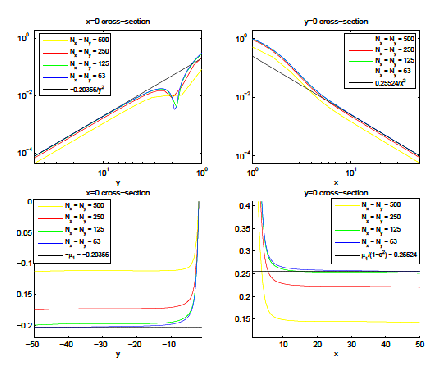
\includegraphics[width=0.98\linewidth]{figure1.eps}   
        \caption{The effect of the mesh size. Upper pannels: funtion $\widehat{U}$  Lower panels: $\tilde r^2 \widehat{U}$  }
	\label{fig1}
\end{figure}

Further on Figure 2 one could see the shape of the solution for different parameters $\tilde c$ and $\beta$:
 
\begin{figure}[htbp]
        \centering
              
\includegraphics[width=0.98\linewidth]{figure2.eps}   
        \caption{Figure 2. 2D and 3D solitonic shapes in a localized domain  $[-10, 10] x [-10, 10]$.}
	\label{fig1}
\end{figure}

%%%%%%%% Section 4 %%%%%%%%%%%%%%%%%%%%
\section{Conclusion}
	That the scope of \cite{ref6} and \cite{ref10} focuses on small phase speeds c and non-uniform grid. The function \ref{ eqBCVC} has small impact on the solution forms obtained in those articles and therefore the observations and results discussed here do not contradict to the outcome obtained in \cite{ref6} and \cite{ref10}. Nevertheless the hyperbolic problem \ref{eq1} with larger phase speed c and also the investigation of the energy functionals ??(nqkoq ot tvoite posledni statii) shifts the priorities into a more detailed investigation of the elliptic Boussinesq equations. Our future goal is to show numerically that equation (1.1) governs the overtaking of wave solutions in 2D as shown in the 1D case [8]. In order to achieve that we have cleared out the problems that appear on the computational boundary of the domain.  The obtained analytical formulas (2.6), (2.8) and (3.3) give great advantage for the numerical computation of the stationary Boussinesq soliton for equations (1.2) and  (3.2) respectively. Instead of choosing a bigger domain to represent the zero boundary conditions at infinity one could use either (2.8) or (3.3).

Other results obtained here which concern convergence of the iterative method, shape of the solution, comparison of the numerical solution from the iterative algorithm [9] with the best-fit formula [12] will be discussed in another article.









\begin{definition}
Text of Definition 1.
\end{definition}

\begin{theorem}
Text of Theorem 1.
\end{theorem}

\begin{proof}
The proof of the theorem.
\end{proof}

\begin{corollary}
Text of Corollary 2.
\end{corollary}

%%%%%%%% Section 2 %%%%%%%%%%%%%%%%%%%%
\section{Second Section of the Paper}

Text ... (see \cite{gasrah}, \cite{rosbl}, \cite{Moak})...

%%%%%%%%%%% REFERENCES %%%%%%%%%%%%%%%%
\begin{thebibliography}{99}

%% example for a book
\bibitem{gasrah} G. Gasper, M. Rahman,
{\it Basic Hypergeometric Series}, Cambridge University Press, Cambridge (1990).

%% example for paper in journal
\bibitem{Moak} D.S. Moak,
The $q$-analogue of the Laguerre polynomials, {\it J. Math. Anal. Appl.}, {\bf 81} (1981), 20-47.

\bibitem{ref1} C. I. Christov, An energy-consistent dispersive shallow-water model,  {\it Wave Motion }, 34, (2001) 161 - 174
\bibitem{ref2} Boussinesq, J. (1871). “Theorie de l’intumescence liquide, applelee onde solitaire ou de translation, se propageant dans un canal rectangulaire”,  {\it Comptes Rendus de l’Academie des Sciences } 72: 755-759

\bibitem{ref3} Boussinesq, J. (1872). “Theorie des ondes et des remous qui se propagent le long d’un canal rectangulaire horizontal, en communiquant au liquide contenu dans ce canal des vitesses sensiblement pareilles de la surface au fond”, {\it Journal de Mathematiques Pures et Aplliquees}, Deuxieme Serie 17: 55-108

\bibitem{ref4} I. Christov, C.I.Christov, Physical dynamics of quasi-particles in nonlinear wave equations, arxiv.org/pdf/nlin/0612005

\bibitem{ref5} J. K. Perring, T. H. R. Skyrme, A model unified field equation, {\it Nuclear Physics},  31 (1962) p. 550-555 

\bibitem{ref6}  C. I. Christov, Numerical implementation of the asymptotic boundary conditions for steadily propagating 2D solitons of Boussinesq type equations, {\it Mathematics and Computers in simulation}, 82 (2012), p. 1079-1092

\bibitem{ref7}  J. Choudhury, C. Christov, 2D Solitary waves of Boussinesq equation, AIP Conference Proceedings (2005), Volume 755, Issue 1, p. 85 - 90

\bibitem{ref8}  M. Christou, C. I. Christov, Fourier Galerkin method for 2D solitons of Boussinesq equation,  {\it Mathematics and Computers in Simulation} 74 (2007) p. 82 - 92

\bibitem{ref9}   M. Christou, C. I. Christov, Galerkin Spectral Method for the 2D Solitary Waves of Boussinesq Paradigm Equation, AIP Conference Proceedings (2009), Volume 1186, Issue 1, p. 217 - 225

\bibitem{ref10} C. I. Christov, J. Choudhury, Perturbation solution for the 2D Boussinesq equation,{\it Mech. Res. Commun. }, 38 (2011) p. 274 - 281

\bibitem{ref11} B. Engquist and A. Majda, Absorbing boundary conditions for the numerical simulation of waves, {\it Math. Comp.}, 31 (1977), p. 629–651.

\bibitem{ref12}  C. I. Goldstein, A finite element method for solving Helmholtz type equations in waveguides and other unbounded domains, {\it Math. Comp.}, 39 (1982), p. 309–324.

\bibitem{ref13}  H.Han, W. Bao, Error estimates for the finite element approximation of problems in unbounded domains,  {\it SIAM J. NUMER. ANAL.} 37, No. 4, p. 1101–1119

\bibitem{ref14} N. Kolkovska, Two Families of Finite Difference Schemes for Multidimensional Boussinesq Paradigm Equation, AIP Conference Proceedings (2010), Volume 1301, p. 395 http://dx.doi.org/10.1063/1.3526638

\bibitem{ref15} N. Kolkovska, K. Angelow, Numerical Computation of the Critical Energy Constant for Two-dimensional Boussinesq Equations,  AIP Conference Proceedings, Volume 1684, 080007-1–080007-6; doi: 10.1063/1.4934318

\bibitem{ref16} P.Northrop, P.A.Ramachandran, W.Schiesser, V. R.Subramanian, A robust false transient method of lines for elliptic partial differential equations, Chemical Engineering Science 90 (2013) 32–39

\bibitem{ref17}
B.~Fornberg, Generation of Finite Difference Formulas on Arbitrarily Spaced Grids, 
{\it  Math. Comput.} , 51(1988),  699 -- 706.

%% example for paper in Proc. or Collected Works
\bibitem{rosbl} M. Rosenblum,
Generalized Hermite polynomials and the Bose-like oscillator
calculus, In: {\it Operator Theory: Advances and Applications},
Birkh\"auser, Basel (1994), 369-396.

\end{thebibliography}

\end{document}
%%%%%%%%%%%%%%%%%%%%%%%%%55
